\documentclass[english, fontsize=12pt, paper=a4, twoside=false, draft=true, pagesize=auto, version=last, DIV=16]{scrartcl}


\let\counterwithout\relax
\let\counterwithin\relax

\usepackage[utf8]{inputenc}
%Für Tabellen
\usepackage{tabularx}

% Für Absätze in Bildbeschreibung
\usepackage{caption}

% Zur nummerierten Aufzählung, mit automatischem Einrücken
\usepackage{paralist}
\usepackage{enumitem}
\usepackage{csquotes}


% mitwachsender Implikationspfeil mit Text
\makeatletter
\newcommand{\xRightarrow}[2][]{\ext@arrow 0359\Rightarrowfill@{#1}{#2}}
\makeatother


% Java Code Einbinden
\usepackage{listings}
\usepackage{color}
\usepackage[svgnames]{xcolor}



% Um einzelne Seiten zu drehen
\usepackage{pdflscape}
%\usepackage{rotating}
%\usepackage{lscape}


\usepackage{lmodern}
\usepackage[T1]{fontenc}
%\usepackage[latin1]{inputenc}
\usepackage{babel}
\usepackage[utf8]{inputenc}
\usepackage{stmaryrd}
\usepackage{extarrows}
\usepackage{ulem}



%Zur Bildnummerierung
\usepackage{chngcntr}
\usepackage{mathtools}
\usepackage{amsmath}
%Zur Verwendung von "chngcntr": \counterwithin{figure}{section}


%Euro-Zeichen
\usepackage{eurosym}

\usepackage{float}

\usepackage{amsmath}
\usepackage{acronym} %[''Optionen'']
\usepackage{esvect}  %Für Vektorpfeile, Aufruf mit \vv{Vektorname}

% Für schön Buchstaben1
\usepackage{mathrsfs}
\usepackage{suetterl}
\usepackage{calligra}

% Einzelne Seite drehen
\usepackage{lscape}


% ----------------------------------------------------------------------------------------
% ----------------------------------- Beginn Code einbinden ------------------------------
% ----------------------------------------------------------------------------------------
% Default fixed font does not support bold face
\DeclareFixedFont{\ttb}{T1}{txtt}{bx}{n}{12} % for bold
\DeclareFixedFont{\ttm}{T1}{txtt}{m}{n}{12}  % for normal

% Custom colors
\usepackage{color}
\definecolor{deepblue}{rgb}{0,0,0.5}
\definecolor{deepred}{rgb}{0.6,0,0}
\definecolor{deepgreen}{rgb}{0,0.5,0}

\usepackage{listings}

% Python style for highlighting
\newcommand\pythonstyle{\lstset{
language=Python,
basicstyle=\fontsize{10}{10}\selectfont\ttfamily,  % oder \ttm, 
otherkeywords={self},             % Add keywords here
keywordstyle=\ttb\color{deepblue},
emph={MyClass,__init__},          % Custom highlighting
emphstyle=\ttb\color{deepred},    % Custom highlighting style
stringstyle=\color{deepgreen},
frame=tb,                         % Any extra options here
showstringspaces=false            % 
}}


% Python environment
\lstnewenvironment{python}[1][]
{
\pythonstyle
\lstset{#1}
}
{}

% Python for external files
\newcommand\pythonexternal[2][]{{
\pythonstyle
\lstinputlisting[#1]{#2}}}


% ----------------------------------------------------------------------------------------
% ------------------------------------ Ende Code einbinden -------------------------------
% ----------------------------------------------------------------------------------------



%%% Neue Kommandos/Begriffe %%%
%\renewcommand{\thesection}{\arabic{section}}
% Für Fußnoten ohne Nummer
%\renewcommand{\thefootnote}{}


% For Citations, comment out if you do not use biber
\usepackage[
	backend=biber,
	style=alphabetic,
	sorting=nty
]{biblatex}
\addbibresource{bib.bib}


% Für die Normalschrift im Abkürzungsverzeichnis, das Paket "acronym" veranlasst eine andere Schriftart bei Abkürzungen.
\newcommand{\Rule}{\rule{\textwidth}{0.5mm}}
% \newcommand{\absatzParagraph}[1]{\paragraph{#1}\mbox{}\\}


\usepackage{geometry}
\newgeometry{left=18mm,right=18mm,top=15mm,bottom=15mm}
\footskip = 22pt

\usepackage{setspace}  % Paket einbinden
\onehalfspacing        % einstellen des Zeilenabstandes auf 1,5
\setlength{\parindent}{0in}
\usepackage{amsmath}
\usepackage[amsmath,amsthm,thmmarks]{ntheorem}
\usepackage{amssymb}


% Komplexitätsklassen
% \usepackage[bold,full]{complexity}


% Für Pseudocode
\usepackage{algorithm}
\usepackage{algpseudocode}


% für mehrzeilige Kommentare
\usepackage{verbatim}


% ------------- Beginn Definition von: Satz, Lemma Definition usw. -------------
\theoremstyle{break}
%\theoremstyle{definition}
\theorembodyfont{\upshape}
\newtheorem{defin}{Definition}[section] % Präambel
\newtheorem{lemma}[defin]{Lemma}
\newtheorem{satz}[defin]{Satz}
\newtheorem{kor}[defin]{Korollar}
\newtheorem{beo}[defin]{Beobachtung}
\newtheorem{bemerk}[defin]{Bemerkung}
\newtheorem{übung}[defin]{Übung}

%  ------------- Ende Definition von: Satz, Lemma Definition usw. -------------

% Für URLs
\usepackage{url}
\usepackage{hyperref}
\hypersetup{final}



\usepackage{animate}
\usepackage{graphicx}
\usepackage{graphics}
\usepackage{hyphenat}


\usepackage{tikz}
\usepackage{tkz-euclide}
%\usepackage{tikz,fullpage}
\usetikzlibrary{calc,patterns,through,intersections}
%\usepackage{tkz-berge}

\newcommand*\bigO{\mathcal{O}}



\begin{document}


\title{
\vspace*{-10mm}
Exercise 3 \\[-3pt]
{\Large $\mathrm{for \ the \ lecture}$} \\[-3pt]
{\LARGE \textbf{Computational Geometry}}
}
\author{Dominik Bendle, Stefan Fritsch, Marcel Rogge and Matthias Tschöpe}
\maketitle
\vspace*{-10mm}

\section*{Exercise 1 (Doubly-Connected Edge List) {\large \hfill (2 + 1 + 1 points)}}
\textbf{a)} Which of the following equations are always true?. 
\begin{align}
\text{Twin}(\text{Twin}(\vec{e})) = \vec{e} \\
\text{Next}(\text{Prev}(\vec{e})) = \vec{e} \\
\text{Twin}(\text{Prev}(\text{Twin}(\vec{e}))) = \text{Next}(\vec{e}) \\
\text{IncidentFace}(\vec{e}) = \text{IncidentFace}(\text{Next}(\vec{e}))
\end{align} \par
\medskip
(1) True. See definition of Twin. \\
(2) True. See definitions of Prev and Next. \\
(3) False. Consider figure \ref{fig:task_1_example} as counterexample, with $\vec{e} := \vec{e}_{2,2}.$
\begin{align*}
&\text{Twin}(\text{Prev}(\text{Twin}(\vec{e}))) \\
= &\text{Twin}(\text{Prev}(\text{Twin}(\vec{e}_{2,2})))\\
= &\text{Twin}(\text{Prev}(\vec{e}_{2,1})) \\
= &\text{Twin}(\vec{e}_{4,2}) \\
= & \vec{e}_{4,1}\\
\neq & \vec{e}_{3,1}\\
= &\text{Next}(\vec{e}_{2,2}) \\
\end{align*}

(4) True. See defintion of IncidentFace. \\

\vspace*{10mm}
\newpage
\begin{figure}[t]
\centering
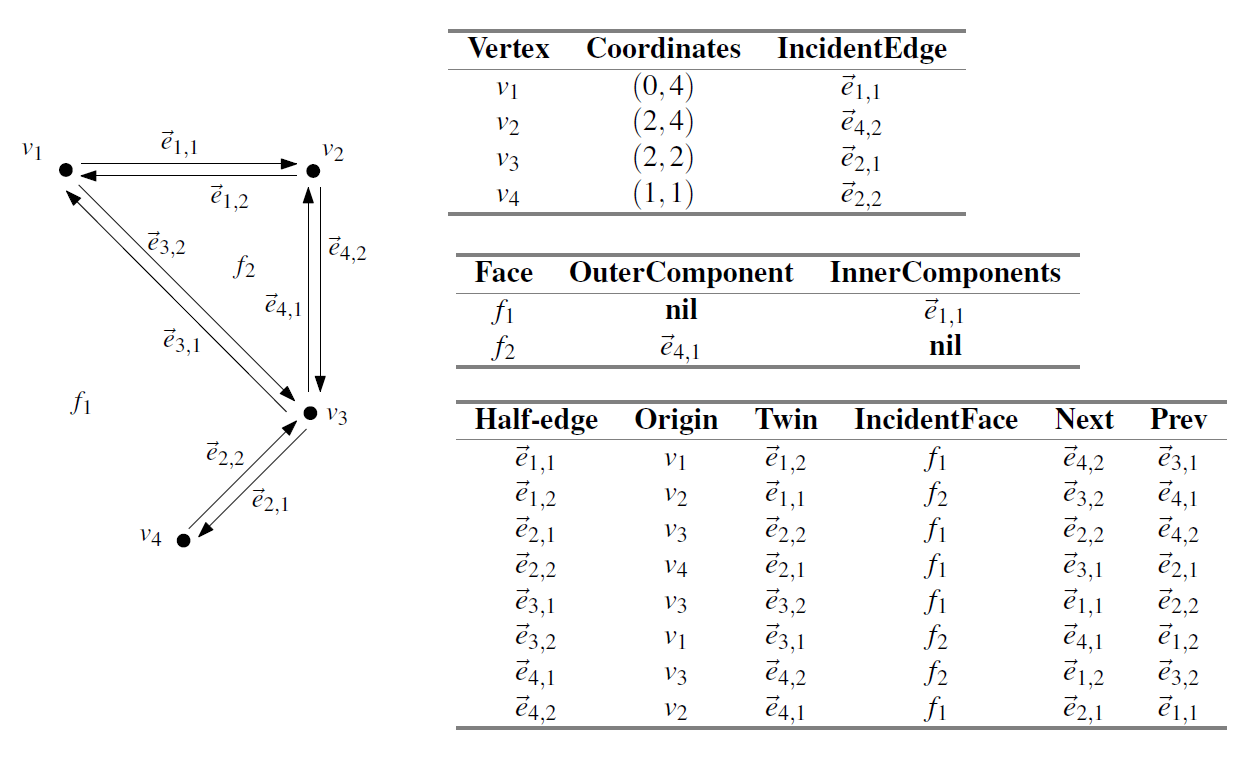
\includegraphics[width=\textwidth]{images/task_1_example.png}
\caption{An example of a doubly-connected edge list for a simple subdivision. Figure is taken from \cite{berg2008computational}.}
\label{fig:task_1_example}
\end{figure}

\textbf{b)} Give an example of a doubly-connected edge list where for an edge $\vec{e}$ the faces IncidentFace($\vec{e}$) and IncidentFace(Twin($\vec{e}$)) are the same. \par
\medskip
Consider this example: \\
\begin{figure}[h]
\centering
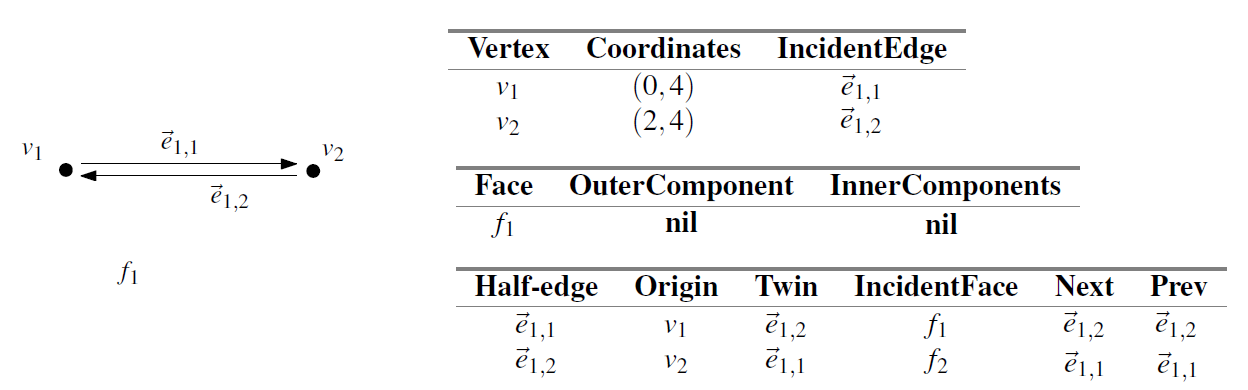
\includegraphics[width=\textwidth]{images/task_1_b.png}
\caption{A very simple example of a doubly-connected edge list.}
\label{fig:task_1_b}
\end{figure}

This is a doubly-connected edge list where $f_1 = \text{IncidentFace}(\vec{e}_{1,1}) = \text{IncidentFace}(\text{Twin}(\vec{e}_{1,1})) = \text{IncidentFace}(\text{Twin}(\vec{e}_{1,2})) = \text{IncidentFace}(\vec{e}_{1,2}) = f_1 $ holds.

\vspace*{10mm}
\newpage

\textbf{c)} Given a doubly-connected edge list representation for a subdivision where
\begin{align*}
\text{Twin}(\vec{e}) = \text{Next}(\vec{e})
\end{align*} 
holds for every half-edge $\vec{e}$. How many faces can the subdivision have at most? \par
\medskip
In this case we have exactly 1 unbounded face. There are only doubly-connected edges like in figure \ref{fig:task_1_b} because this is the only case where $\text{Twin}(\vec{e}) = \text{Next}(\vec{e})$ holds. (Of course we might have many of these edges and some of them might be sharing some nodes). By definition each half-edge bounds only one face. We can easily apply the prove from \textbf{b)} here and use it to show that this is always the same face. This shows that there can only be exactly 1 unbounded face.

\vspace*{10mm}
\newpage




\section*{Exercise 2 (Planar Subdivision and Point Set) {\large \hfill (4 points)}}

Let S.vertices be a list of vertices, which has the always the edge in counter-clockwise direction as incident face. The edges in counter-clockwise direction are the inner edges.\\

V = sort(S.vertices)\\
F = [ ]\\

for p $\in$ P\\
\hspace*{10mm}face = null\\
\hspace*{10mm}vertices = V\\
\hspace*{10mm}while size(vertices) > 0\\
\hspace*{10mm}\hspace*{10mm}current\_face = null\\
\hspace*{10mm}\hspace*{10mm}v = vertices.pop()\\
\hspace*{10mm}\hspace*{10mm}i = v.incident\_edge\\
\hspace*{10mm}\hspace*{10mm}n = i.next\_edge\\
\hspace*{10mm}\hspace*{10mm}if is\_left(point, i)\\
\hspace*{10mm}\hspace*{10mm}\hspace*{10mm}current\_face = i.incident\_face\\
\hspace*{10mm}\hspace*{10mm}while i != n\\
\hspace*{10mm}\hspace*{10mm}\hspace*{10mm}vertices.remove(n.origin)\\
\hspace*{10mm}\hspace*{10mm}\hspace*{10mm}if current\_face != null\\
\hspace*{10mm}\hspace*{10mm}\hspace*{10mm}\hspace*{10mm}if is\_right(point, n)\\
\hspace*{10mm}\hspace*{10mm}\hspace*{10mm}\hspace*{10mm}\hspace*{10mm}current\_face = null\\
\hspace*{10mm}\hspace*{10mm}\hspace*{10mm}n = n.next\_edge\\
\hspace*{10mm}\hspace*{10mm}if current\_face != null\\
\hspace*{10mm}\hspace*{10mm}\hspace*{10mm}face = current\_face\\
\hspace*{10mm}F.append(face)\\

F lists the face in which each point lies. If a face is null, that means the point lies outside of all polygons.\\
The complexity of this algorithm is n*m, as for each of the m points, each of the n edges has to be checked.

\newpage

\section*{Exercise 3 (Planar Subdivision and Point Set) {\large \hfill (1 points)}}

\section*{Exercise 4 (Planar Subdivision and Point Set) {\large \hfill (1 points)}}

\newpage


\begin{landscape}
\section*{Exercise 5 (3-Coloring of Simple Polygons) {\large \hfill (5 points)}} 
For saving space, we only hand in our function for computing the 3-coloring, and skip all helper functions like reading the ply files or drawing the results. We encode all three colors by the numbers 0, 1 and 2. After that, we encode those numbers by real colors. But this is not part of this function. \par
\bigskip

\begin{python}
# tri is the abbreviation of triangle.
def coloring(tri, colors, next_triangle, used_triangle):
    if tri != []:
        p1 = tri[next_triangle][0]
        p2 = tri[next_triangle][1]
        p3 = tri[next_triangle][2]

        used_triangle[next_triangle] = 1

        # This can only be true in the first call of coloring(), because initial are all colors -1
        if max(colors) == -1:
            colors[p1] = 0
            colors[p2] = 1

        if colors[p1] == -1 and colors[p2] != -1 and colors[p3] != -1:
            all_possible_colors = [0,1,2]
            all_possible_colors.remove(colors[p2])
            all_possible_colors.remove(colors[p3])
            colors[p1] = all_possible_colors[0]

        if colors[p2] == -1 and colors[p1] != -1 and colors[p3] != -1:
            all_possible_colors = [0,1,2]
            all_possible_colors.remove(colors[p1])
            all_possible_colors.remove(colors[p3])
            colors[p2] = all_possible_colors[0]

        if colors[p3] == -1 and colors[p1] != -1 and colors[p2] != -1:
            all_possible_colors = [0,1,2]
            all_possible_colors.remove(colors[p1])
            all_possible_colors.remove(colors[p2])
            colors[p3] = all_possible_colors[0]
            
        p1_p2_triangles = [i for i in range(len(tri)) if p1 in tri[i] and p2 in tri[i] and not p3 in tri[i]]
        p1_p3_triangles = [i for i in range(len(tri)) if p1 in tri[i] and p3 in tri[i] and not p2 in tri[i]]
        p2_p3_triangles = [i for i in range(len(tri)) if p2 in tri[i] and p3 in tri[i] and not p1 in tri[i]]

        children = p1_p2_triangles + p1_p3_triangles + p2_p3_triangles

        for face in children:
            if used_triangle[face] != -1:
                children.remove(face)

        for child in children:
            coloring(tri, colors, child, used_triangle)

    else:
        if min(colors) == -1:
            coloring(tri, colors, 0, used_triangle)

    return colors
\end{python}
\end{landscape}
\newpage

\begin{figure}[h!]
\centering
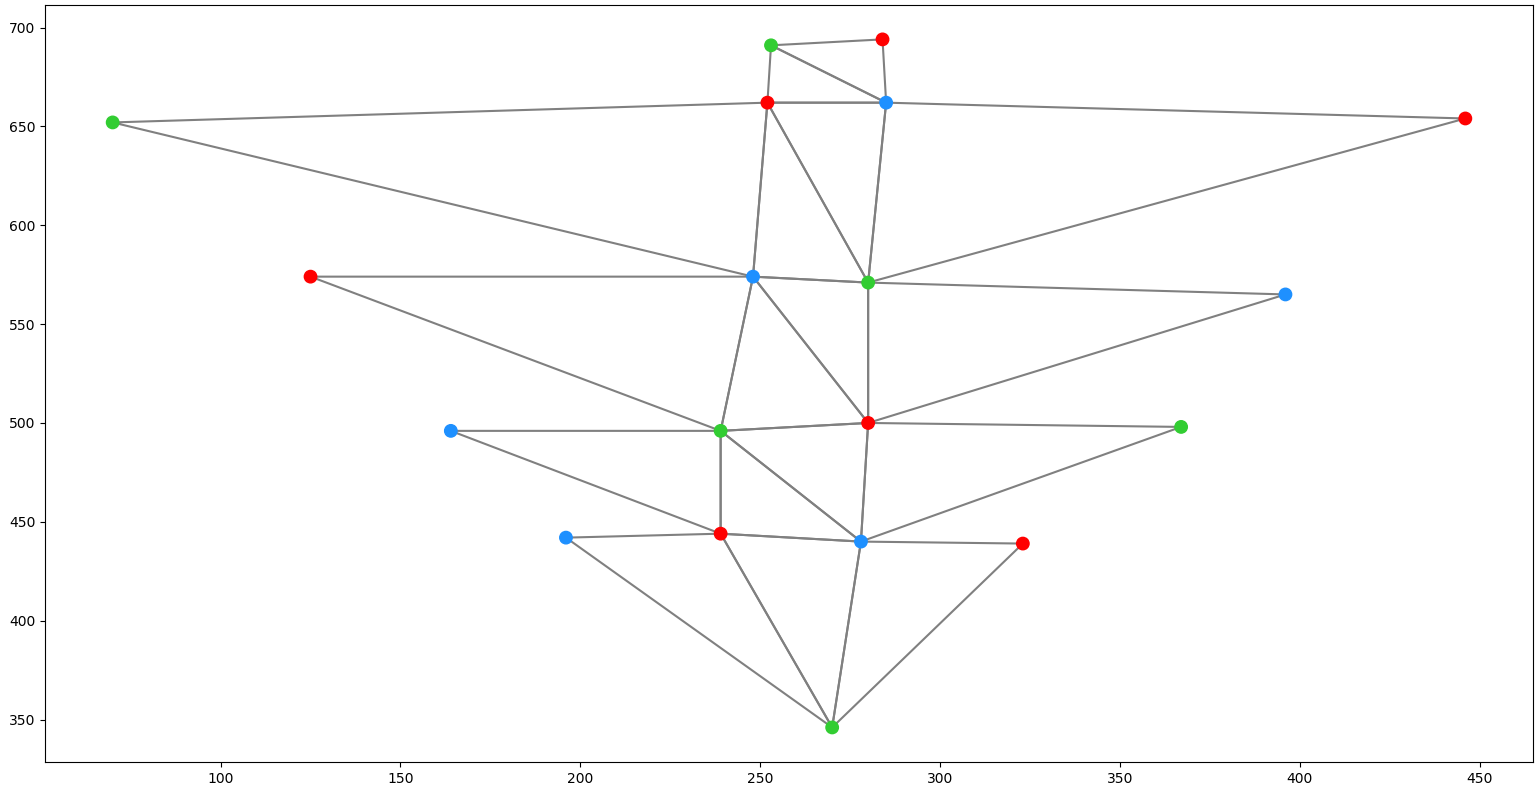
\includegraphics[width=\textwidth]{images/Figure_1.png}
\caption{3-coloring of the dataset: simplePolygonTriangulated\_1.ply.}
\label{fig:task_1_b}
\end{figure}
\vspace*{15mm}

\begin{figure}[h!]
\centering
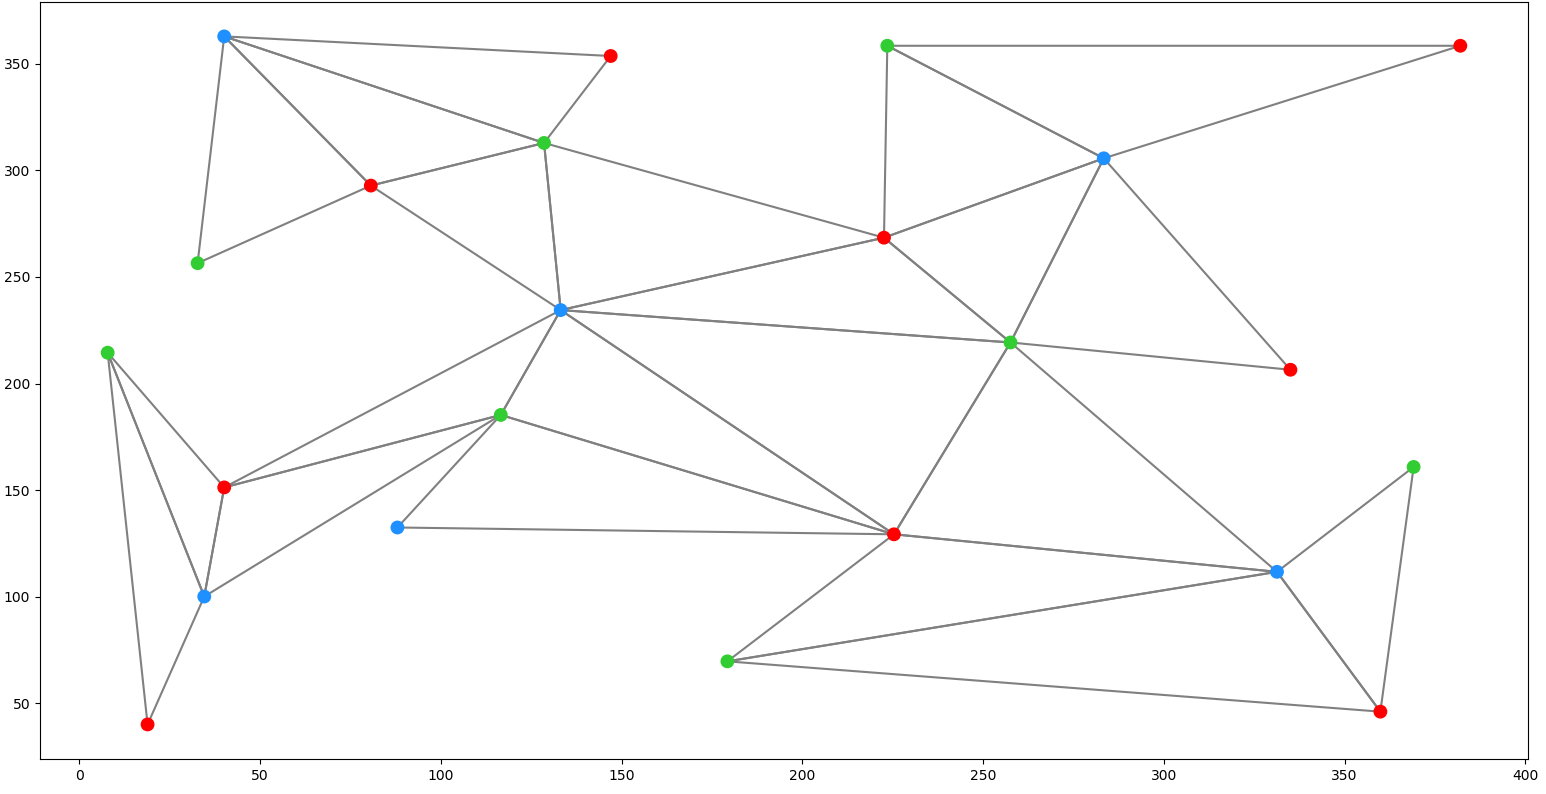
\includegraphics[width=\textwidth]{images/Figure_2.png}
\caption{3-coloring of the dataset: simplePolygonTriangulated\_2.ply.}
\label{fig:task_1_b}
\end{figure}



% ---- Bibliography ----
% Vermutlich ohne Biber:
% \bibliographystyle{plain}
% \bibliography{bib}
	
% Mit Biber
\printbibliography
%
\end{document}



